本章节是Thomas R . Kane的《Spacecraft Dynamics》一书第一章还有张建书老师文档的学习笔记.
\section{简单转动}

\begin{mydefinition}{简单转动}
若存在一条称为转轴的直线$L$，其相对于刚体或参考系$A$的取向在整个运动过程中保持不变，和刚体或参考系$B$的取向在整个运动过程中保持不变，则刚体或参考系$B$相对于刚体或参考系$A$的运动称为$B$在$A$中的简单转动。
\end{mydefinition}

设$\boldsymbol{a}$为$A$中的一个向量.$\boldsymbol{b}$为$B$中的一个向量，且在转动之前与$\boldsymbol{a}$重合，则满足如下关系：
\begin{equation}\label{eq:simple_rotation_formula}
\boldsymbol{b} = \boldsymbol{a}\cos\theta - (\boldsymbol{a}\times\boldsymbol{\lambda})\sin\theta + \boldsymbol{\lambda}(\boldsymbol{\lambda}\cdot\boldsymbol{a})(1-\cos\theta)
\end{equation}

如果一个矩阵定义为：
\begin{equation}
    \boldsymbol{A} \triangleq \boldsymbol{U}\cos\theta - (\boldsymbol{U}\times\boldsymbol{\lambda})\sin\theta + \boldsymbol{\lambda}(\boldsymbol{\lambda}\cdot\boldsymbol{U})(1-\cos\theta)
\end{equation}

则有：
\begin{equation}
    \boldsymbol{b} = \boldsymbol{a}\cdot\boldsymbol{A}
\end{equation}

\begin{proof}
设$\boldsymbol{\alpha_{1}}$,$\boldsymbol{\alpha_{2}}$为坐标系$A$中的两个单位向量，且满足：
$$
    \boldsymbol{\alpha_{1}}\parallel L_{A}
$$
$$
\boldsymbol{\alpha_{2}}=\boldsymbol{\lambda}\times\boldsymbol{\alpha_{1}}
$$

设$\boldsymbol{\beta_{1}}$,$\boldsymbol{\beta_{2}}$为坐标系$B$中的两个单位向量，且满足：
$$
    \boldsymbol{\beta_{1}}\parallel L_{B}
$$
$$
\boldsymbol{\beta_{2}}=\boldsymbol{\lambda}\times\boldsymbol{\beta_{1}}
$$
且满足，当转角$\theta=0$时，有：
$$\boldsymbol{a}=\boldsymbol{b}$$
$$
    \boldsymbol{\alpha_{1}}=\boldsymbol{\beta_{1}}
$$
$$
\boldsymbol{\alpha_{2}}=\boldsymbol{\beta_{2}}
$$
\begin{figure}[htbp]
    \centering
    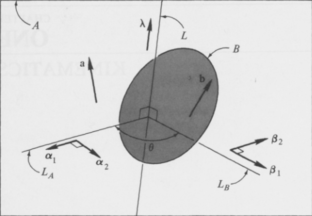
\includegraphics[width=0.8\textwidth]{Figure/1.1简单转动.png}
    \caption{简单转动}
    \label{fig:simple_rotation}
\end{figure}

那么，$\boldsymbol{a}$和$\boldsymbol{b}$可以表示为：
$$\boldsymbol{a}=p\boldsymbol{\alpha_{1}}+q\boldsymbol{\alpha_{2}}+r\boldsymbol{\lambda}$$
$$\boldsymbol{b}=p\boldsymbol{\beta_{1}}+q\boldsymbol{\beta_{2}}+r\boldsymbol{\lambda}$$

且有关系：
$$\boldsymbol{\beta_{1}}=\cos\theta\boldsymbol{\alpha_{1}}+\sin\theta\boldsymbol{\alpha_{2}}$$
$$\boldsymbol{\beta_{2}}=-\sin\theta\boldsymbol{\alpha_{1}}+\cos\theta\boldsymbol{\alpha_{2}}$$
代入即可得式子\eqref{eq:simple_rotation_formula}
\end{proof}


\section{方向余弦}
当我们进行坐标变换时，我们需要使用方向余弦矩阵来表示坐标变换的矩阵形式。
我们一定可以得到这样的式子：
\begin{equation}
    \left\{\begin{array}{l}
\mathbf{e}_{1|A} = a_{11}\,\mathbf{e}_{1|B} + a_{12}\,\mathbf{e}_{2|B} + a_{13}\,\mathbf{e}_{3|B},\\
\mathbf{e}_{2|A} = a_{21}\,\mathbf{e}_{1|B} + a_{22}\,\mathbf{e}_{2|B} + a_{23}\,\mathbf{e}_{3|B},\\
\mathbf{e}_{3|A} = a_{31}\,\mathbf{e}_{1|B} + a_{32}\,\mathbf{e}_{2|B} + a_{33}\,\mathbf{e}_{3|B}.
\end{array}\right.
\end{equation}
\begin{equation}
    \begin{bmatrix}\boldsymbol{e}_{1}\\\boldsymbol{e}_{2}\\\boldsymbol{e}_{3}\end{bmatrix}_A=\begin{bmatrix}a_{11}&a_{12}&a_{13}\\a_{21}&a_{22}&a_{23}\\a_{31}&a_{32}&a_{33}\end{bmatrix}_{AB}\begin{bmatrix}\boldsymbol{e}_{1}\\\boldsymbol{e}_{2}\\\boldsymbol{e}_{3}\end{bmatrix}_B
\end{equation}
\begin{mydefinition}{方向余弦}
设 $\boldsymbol{e}_{1|A}, \boldsymbol{e}_{2|A}, \boldsymbol{e}_{3|A}$ 为 $A$ 中的三个互相垂直的单位向量，$\boldsymbol{e}_{1|B}, \boldsymbol{e}_{2|B}, \boldsymbol{e}_{3|B}$ 为 $B$ 中的三个互相垂直的单位向量，则 $\boldsymbol{e}_{i|A}$ 在 $B$ 中沿 $\boldsymbol{e}_{j|B}$ 的方向余弦定义为：
$$
a_{ij}\triangleq\mathbf{e}_{i|A}\cdot\mathbf{e}_{j|B}\quad(i,j=1,2,3)
$$
\end{mydefinition}
于是方向余弦矩阵：
\begin{equation}
    \label{eq:direction_cosine_matrix}
    \boldsymbol{A} \triangleq
    \begin{bmatrix}
        a_{11} & a_{12} & a_{13} \\
        a_{21} & a_{22} & a_{23} \\
        a_{31} & a_{32} & a_{33}
    \end{bmatrix}
\end{equation}

有了方向余弦矩阵的基本概念之后，我们来讨论方向余弦矩阵的基本性质。
\subsubsection{方向余弦矩阵的基本性质}
\begin{myTheorem}{性质一：投影变换}
    设$\mathbf{v_A}$,$\mathbf{v_B}$分别为$A$和$B$中的向量，且为$\mathbf{v}$在$A$和$B$中的投影，则有：
$$\mathbf{v_A}=\boldsymbol{A}\mathbf{v_B}$$

\end{myTheorem}

\begin{myTheorem}{性质二}
    两个方向相同的坐标系之间的方向余弦矩阵为单位矩阵
\end{myTheorem}

\begin{myTheorem}{性质三}
    方向余弦矩阵中的 9 个数满足 6 个独立的约束方程.
\end{myTheorem}
\begin{proof}
    用坐标系B中的矢量基表示坐标系A中的矢量基：
     $$\begin{bmatrix}\boldsymbol{e}_{1}\\\boldsymbol{e}_{2}\\\boldsymbol{e}_{3}\end{bmatrix}_A=\begin{bmatrix}a_{11}&a_{12}&a_{13}\\a_{21}&a_{22}&a_{23}\\a_{31}&a_{32}&a_{33}\end{bmatrix}_{AB}\begin{bmatrix}\boldsymbol{e}_{1}\\\boldsymbol{e}_{2}\\\boldsymbol{e}_{3}\end{bmatrix}_B$$
     满足两组约束方程：

     (\uppercase\expandafter{\romannumeral1})A系坐标轴上的单位矢量模为1：$$\begin{cases}&|\boldsymbol{e}_{1|A}|=\sqrt{a_{11}^2+a_{12}^2+a_{13}^2}=1,\\&|\boldsymbol{e}_{2|A}|=\sqrt{a_{21}^2+a_{22}^2+a_{23}^2}=1,\\&|\boldsymbol{e}_{3|A}|=\sqrt{a_{31}^2+a_{32}^2+a_{33}^2}=1.\end{cases}$$


     (\uppercase\expandafter{\romannumeral2})A系坐标轴上的单位矢量两两正交:$$\begin{cases}&\boldsymbol{e}_{1|A}\cdot\boldsymbol{e}_{2|A}=a_{11}a_{21}+a_{12}a_{22}+a_{13}a_{23}=0,\\&\boldsymbol{e}_{1|A}\cdot\boldsymbol{e}_{3|A}=a_{11}a_{31}+a_{12}a_{32}+a_{13}a_{33}=0,\\&\boldsymbol{e}_{2|A}\cdot\boldsymbol{e}_{3|A}=a_{21}a_{31}+a_{22}a_{32}+a_{23}a_{33}=0.\end{cases}$$


\end{proof}
\begin{myTheorem}{性质四}
    方向余弦矩阵等于其余子矩阵，即方向余弦矩阵中的每个数都等于其对应的代数余子式，即：
    \begin{equation}
        \begin{bmatrix}a_{11}&a_{12}&a_{13}\\a_{21}&a_{22}&a_{23}\\a_{31}&a_{32}&a_{33}\end{bmatrix}_{AB}=\begin{bmatrix}\begin{vmatrix}a_{22}&a_{23}\\a_{32}&a_{33}\end{vmatrix}&-\begin{vmatrix}a_{21}&a_{23}\\a_{31}&a_{33}\end{vmatrix}&\begin{vmatrix}a_{21}&a_{22}\\a_{31}&a_{32}\end{vmatrix}\\-\begin{vmatrix}a_{12}&a_{13}\\a_{32}&a_{33}\end{vmatrix}&\begin{vmatrix}a_{11}&a_{13}\\a_{31}&a_{33}\end{vmatrix}&-\begin{vmatrix}a_{11}&a_{12}\\a_{31}&a_{32}\end{vmatrix}\\\begin{vmatrix}a_{12}&a_{13}\\a_{22}&a_{23}\end{vmatrix}&-\begin{vmatrix}a_{11}&a_{13}\\a_{21}&a_{23}\end{vmatrix}&\begin{vmatrix}a_{11}&a_{12}\\a_{21}&a_{22}\end{vmatrix}\end{bmatrix}_{AB}.
    \end{equation}
\end{myTheorem}

\begin{proof}
    依旧用坐标系B中的矢量基表示坐标系A中的矢量基：
     $$\begin{bmatrix}\boldsymbol{e}_{1}\\\boldsymbol{e}_{2}\\\boldsymbol{e}_{3}\end{bmatrix}_A=\begin{bmatrix}a_{11}&a_{12}&a_{13}\\a_{21}&a_{22}&a_{23}\\a_{31}&a_{32}&a_{33}\end{bmatrix}_{AB}\begin{bmatrix}\boldsymbol{e}_{1}\\\boldsymbol{e}_{2}\\\boldsymbol{e}_{3}\end{bmatrix}_B$$

     我们知道，A系坐标轴上的单位矢量两两正交，所以有：
    \begin{equation}
    \begin{aligned}
        \boldsymbol{e}_{1|A}&=\boldsymbol{e}_{2|A}\times\boldsymbol{e}_{3|A}\\
        &=\begin{vmatrix}\boldsymbol{e}_{1|B}&\boldsymbol{e}_{2|B}&\boldsymbol{e}_{3|B}\\a_{11}&a_{12}&a_{13}\\a_{21}&a_{22}&a_{23}\end{vmatrix}\\
        &=\begin{vmatrix}a_{22}&a_{23}\\a_{32}&a_{33}\end{vmatrix}\boldsymbol{e}_{1|B}-\begin{vmatrix}a_{21}&a_{23}\\a_{31}&a_{33}\end{vmatrix}\boldsymbol{e}_{2|B}+\begin{vmatrix}a_{21}&a_{22}\\a_{31}&a_{32}\end{vmatrix}\boldsymbol{e}_{3|B}
    \end{aligned}
    \end{equation}

\end{proof}


\begin{myTheorem}{性质五：正交性}
    方向余弦矩阵是正交矩阵，即：
$$\boldsymbol{A}^{-1} = \boldsymbol{A}^{T}$$
        $$\boldsymbol{A}^{T}\boldsymbol{A}=\boldsymbol{I}$$

\end{myTheorem}
\begin{proof}
    设$\mathbf{v_A}$,$\mathbf{v_B}$分别为$A$和$B$中的向量，且为$\mathbf{v}$在$A$和$B$中的投影，则有：
$$\mathbf{v_A}=\boldsymbol{A}\mathbf{v_B}$$
    由于$\mathbf{v_A}$,$\mathbf{v_B}$为同一个向量在不同坐标系下的投影，所以有：
$$\mathbf{v_A}\cdot\mathbf{v_A}=\mathbf{v_B}\cdot\mathbf{v_B}$$
    代入上式可得：
$$\mathbf{v_B}^{T}\boldsymbol{A}^{T}\boldsymbol{A}\mathbf{v_B}=\mathbf{v_B}^{T}\mathbf{v_B}$$
    由于$\mathbf{v_B}$为任意向量，所以有：
$$\boldsymbol{A}^{T}\boldsymbol{A}=\boldsymbol{I}$$
    于是有：
$$\boldsymbol{A}^{-1} = \boldsymbol{A}^{T}$$
\end{proof}

\begin{myTheorem}{性质六}
    方向余弦矩阵行列式的值为正 1.
\end{myTheorem}
\begin{proof}
    由性质四，还有按照行列式运算的按第一行展开即可。
\end{proof}

\begin{myTheorem}{性质七}
    同一矢量$\mathbf{v}$在 A 中的投影列阵$\mathbf{v_A}$对应的叉乘矩阵$\tilde{\mathbf{v}}_A$和它在 B 系中的投影列阵$\mathbf{v_B}$对应的叉乘矩阵$\tilde{\mathbf{v}}_B$之间满足如下坐标变换式和它在 B 系中的投影列阵$\mathbf{v_B}$对应的叉乘矩阵$\tilde{\mathbf{v}}_B$之间满足如下坐标变换式$$\tilde{\mathbf{v}}_A=\mathbf{A}_{AB}\tilde{\mathbf{v}}_B \mathbf{A}_{AB}^\mathrm{T}$$

    由此可得：
    \begin{equation}
        \mathbf{A}_{AB}^\mathrm{T} \tilde{\mathbf{v}}_A=\tilde{\mathbf{v}}_B \mathbf{A}_{AB}^\mathrm{T}
    \end{equation}
    和
    \begin{equation}
        \tilde{\mathbf{v}}_A\mathbf{A}_{AB}=\mathbf{A}_{AB}\tilde{\mathbf{v}}_B
    \end{equation}

\end{myTheorem}


\begin{myTheorem}{性质八}
    任意两个坐标系 i 和 j 之间的方向余弦矩阵$\mathbf{A}_{ij}$ 都有一个实特征值1，即存在一个实数形式的特征向量$\mathbf{\lambda}$, 该特征向量满足$\mathbf{\lambda}=\mathbf{A}_{ij}\mathbf{\lambda}$. 该性质表明两坐标间的任意相对转动都可以通过一次定轴 (简单) 转动来完成
\end{myTheorem}

\begin{figure}[htbp]
    \centering
    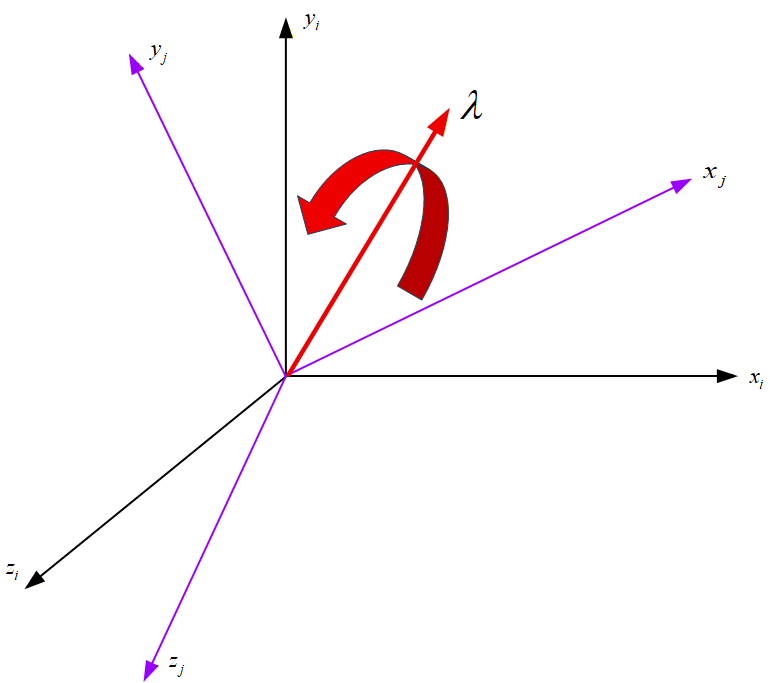
\includegraphics[width=0.6\textwidth]{Figure/简单旋转示意图.png}
    \caption{简单旋转示意图}
    \label{fig:简单旋转示意图}
\end{figure}

\begin{proof}
    由特征多项式的定义：
    \[
    f_{\boldsymbol{A}}(\lambda) \triangleq \det(\boldsymbol{A}-\lambda\boldsymbol{I}_{3})
    \]
    写成显式行列式：
    \[
    =\left|\begin{array}{ccc}
    a_{11}-\lambda & a_{12} & a_{13} \\
    a_{21} & a_{22}-\lambda & a_{23} \\
    a_{31} & a_{32} & a_{33}-\lambda
    \end{array}\right|
    \]

    按第一行余子式展开（cofactor expansion along the first row）：
    \[
    \begin{aligned}
    =&\ (a_{11}-\lambda)\bigl[(a_{22}-\lambda)(a_{33}-\lambda) - a_{23}a_{32}\bigr] \\
    &-\ a_{12}\bigl[a_{21}(a_{33}-\lambda) - a_{23}a_{31}\bigr] \\
    &+\ a_{13}\bigl[a_{21}a_{32} - (a_{22}-\lambda)a_{31}\bigr]
    \end{aligned}
    \]

    记 $M_{kk}$ 为主对角元 $a_{kk}$ 的二阶余子式，即
    \[
    M_{11}=a_{22}a_{33}-a_{23}a_{32},\quad
    M_{22}=a_{11}a_{33}-a_{13}a_{31},\quad
    M_{33}=a_{11}a_{22}-a_{12}a_{21}.
    \]
    将每个二阶行列式用 $M_{kk}$ 与 $\lambda$ 的多项式表示：
    \[
    \begin{aligned}
    (a_{22}-\lambda)(a_{33}-\lambda) - a_{23}a_{32}
        &= M_{11} - (a_{22}+a_{33})\lambda + \lambda^{2} \\
    a_{21}(a_{33}-\lambda) - a_{23}a_{31}
        &= (a_{21}a_{33}-a_{23}a_{31}) - a_{21}\lambda \\
    a_{21}a_{32} - (a_{22}-\lambda)a_{31}
        &= (a_{21}a_{32}-a_{22}a_{31}) + a_{31}\lambda
    \end{aligned}
    \]

    代入并按 $\lambda$ 的幂次合并同类项：
    \[
    \begin{aligned}
    =&\ \underbrace{-\lambda^{3}}_{\text{from }(a_{11}-\lambda)\cdot\lambda^{2}} \\
    &+\ \underbrace{\bigl[a_{11}+(a_{22}+a_{33})\bigr]\lambda^{2}}_{\text{from }(a_{11}-\lambda)\cdot[-(\!a_{22}\!+\!a_{33}\!)\lambda]+\text{其它}} \\
    &-\ \underbrace{\bigl[a_{11}(a_{22}+a_{33})+(a_{22}a_{33}-a_{23}a_{32})-(a_{12}a_{21}+a_{13}a_{31})\bigr]\lambda}_{\text{合并所有 $\lambda^{1}$ 项}} \\
    &+\ \underbrace{(a_{11}a_{22}a_{33}+a_{12}a_{23}a_{31}+a_{13}a_{21}a_{32}-a_{11}a_{23}a_{32}-a_{12}a_{21}a_{33}-a_{13}a_{22}a_{31})}_{\text{常数项}}
    \end{aligned}
    \]

    注意到常数项恰为 $\det\boldsymbol{A}$ 的 Sarrus 展开；$\lambda^{1}$ 系数括号中
    \[
    a_{11}(a_{22}+a_{33})+(a_{22}a_{33}-a_{23}a_{32})-(a_{12}a_{21}+a_{13}a_{31})
    =M_{11}+M_{22}+M_{33}=\sum_{k=1}^{3}M_{kk},
    \]
    $\lambda^{2}$ 系数 $a_{11}+a_{22}+a_{33}=\mathrm{tr}(\boldsymbol{A})$。故可整理为
    \[
    = -\lambda^{3} + \mathrm{tr}(\boldsymbol{A})\,\lambda^{2} - \left(\sum_{k=1}^{3}M_{kk}\right)\lambda + \det(\boldsymbol{A}).
    \]

    对于方向余弦矩阵，由 $\boldsymbol{A}^{T}\boldsymbol{A}=\boldsymbol{I}$ 可得
    \[
    M_{11}+M_{22}+M_{33} = \mathrm{tr}(\boldsymbol{A}),
    \]
    又由性质 $\det\boldsymbol{A}=1$（旋转不改变体积），于是
    \[
    f_{\boldsymbol{A}}(\lambda) = -\lambda^{3} + \mathrm{tr}(\boldsymbol{A})\,\lambda^{2} - \mathrm{tr}(\boldsymbol{A})\,\lambda + 1.
    \]
    将$\lambda=1$代入上式可得：
\[
f_{\boldsymbol{A}}(1) = -1 + \mathrm{tr}(\boldsymbol{A}) - \mathrm{tr}(\boldsymbol{A}) + 1 = 0.
\]
    因此，$\lambda=1$是$f_{\boldsymbol{A}}(\lambda)$的一个根，即$\boldsymbol{A}$有一个实特征值为1
\end{proof}

从高等代数的角度思考一下这个特征值的意义，我们知道，特征值的意义是：
\begin{equation}
    \boldsymbol{A}\mathbf{\lambda}=\mathbf{\lambda}
\end{equation}
也就是说，在本次旋转变换中转轴$\mathbf{\lambda}$并没有发生变化，即转轴朝向不变。

若已知转角$\theta$和转轴$\mathbf{\lambda}$，那我们怎么得出方向余弦矩阵呢？Kane的书里给出了一种计算方法。
\begin{equation}
    \label{eq:方向余弦矩阵计算式}
    \begin{aligned}&a_{11}=\cos\theta+\lambda_1^2(1-\cos\theta)\\&a_{12}=-\lambda_3\sin\theta+\lambda_1\lambda_2(1-\cos\theta)\\&a_{13}=\lambda_2\sin\theta+\lambda_3\lambda_1(1-\cos\theta)\\&a_{21}=\lambda_3\sin\theta+\lambda_1\lambda_2(1-\cos\theta)\\&a_{22}=\cos\theta+\lambda_2^2(1-\cos\theta)\\&a_{23}=-\lambda_1\sin\theta+\lambda_2\lambda_3(1-\cos\theta)\\&a_{31}=-\lambda_2\sin\theta+\lambda_3\lambda_1(1-\cos\theta)\\&a_{32}=\lambda_1\sin\theta+\lambda_2\lambda_3(1-\cos\theta)\\&a_{33}=\cos\theta+\lambda_3^2(1-\cos\theta)
\end{aligned}
\end{equation}
为了方便记忆，引入一个符号$\epsilon_{ijk}$
\begin{equation}
    \epsilon_{ijk}\triangleq\frac{1}{2}(i-j)(j-k)(k-i)\quad(i,j,k=1,2,3)
\end{equation}
这样式~\eqref{eq:方向余弦矩阵计算式}可以写成：
\begin{equation}
    a_{ij}=\delta_{ij}\cos\theta-\epsilon_{ijk}\lambda_{k}\sin\theta+\lambda_{i}\lambda_{j}(1-\cos\theta)\quad(i,j=1,2,3)
\end{equation}

那么这个神奇的式子是怎么得到的呢？
\begin{proof}
    我们知道，$\boldsymbol{e}_{i|A}=\boldsymbol{A}\boldsymbol{e}_{i|B}$,然后还有$a_{ij}=\boldsymbol{e}_{i|A}\cdot\boldsymbol{e}_{j|B}=\boldsymbol{e}_{i|B}\cdot(\boldsymbol{A}\boldsymbol{e}_{j|B})$

    然后又有式~\eqref{eq:simple_rotation_formula}，

$$\boldsymbol{e_A} = \boldsymbol{e_B}\cos\theta - (\boldsymbol{e_B}\times\boldsymbol{\lambda})\sin\theta + \boldsymbol{\lambda}(\boldsymbol{\lambda}\cdot\boldsymbol{e_B})(1-\cos\theta)$$
然后再加上$\boldsymbol{\lambda}_i \triangleq \boldsymbol{\lambda}\cdot\boldsymbol{e}_{i|B}=\boldsymbol{\lambda}\cdot\boldsymbol{e}_{i|A}$
代入即可得到式~\eqref{eq:方向余弦矩阵计算式}
\end{proof}
为了使我们对方向余弦有更好的理解，Kane的书里给出了一个例题。
\begin{example}
    在图~\ref{fig:方向余弦矩阵例题}中，B表示一个均匀矩形块，它是安装在航天器A中的扫描平台的一部分。初始时，B的各条边与固定在A中的单位矢量$\boldsymbol{\alpha_1}, \boldsymbol{\alpha_2}, \boldsymbol{\alpha_3}$平行，随后平台绕B的一条对角线做简单的90度旋转，如示意图所示。设$\mathbf{I}$为刚体B关于其质心B*的惯性并矢.且定义$\mathbf{I}_{ij|A}$为$$\mathbf{I}_{ij|A} \triangleq \boldsymbol{\alpha_i} \cdot \mathbf{I} \cdot \boldsymbol{\alpha_j} \quad(i,j=1,2,3)$$问旋转之后的$\mathbf{I}_{ij|A}\quad(i,j=1,2,3)$为多少？
    \begin{figure}[htbp]
        \centering
        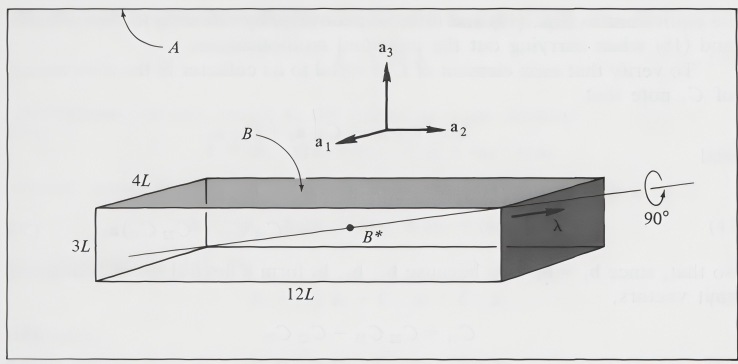
\includegraphics[width=0.8\textwidth]{Figure/例题2.1.png}
        \caption{例题2.1}
        \label{fig:方向余弦矩阵例题}
    \end{figure}
\end{example}
\begin{solution}
    设$\boldsymbol{b_1}, \boldsymbol{b_2}, \boldsymbol{b_3}$为固定在B中的单位向量，旋转前与$\boldsymbol{\alpha_1}, \boldsymbol{\alpha_2}, \boldsymbol{\alpha_3}$相等.

    定义$\mathbf{I}_{ij|B}\triangleq\boldsymbol{b_i} \cdot \mathbf{I} \cdot \boldsymbol{b_j} \quad(i,j=1,2,3)$
    那么$\boldsymbol{b_1}$、$\boldsymbol{b_2}$和$\boldsymbol{b_3}$平行于刚体B对B*点的惯性主轴，因此
    $$\mathbf{I}_{12|B}=\mathbf{I}_{21|B}=\mathbf{I}_{23|B}=\mathbf{I}_{32|B}=\mathbf{I}_{31|B}=\mathbf{I}_{13|B}=0$$
    非主对角线元素均为0，下面计算主对角线元素：
    $$\mathbf{I}_{11|B}=\frac{m}{12}(12^{2}+3^{2})L^{2}=\frac{153}{12}mL^{2}$$
    $$\mathbf{I}_{22|B}=\frac{m}{12}(3^2+4^2)L^2=\frac{25}{12}mL^2$$
    $$\mathbf{I}_{33|B}=\frac{m}{12}(4^2+12^2)L^2=\frac{160}{12}mL^2$$

    于是完整的惯性矩阵：$$\mathbf{I}_B=\frac{mL^2}{12}\begin{bmatrix}153&0&0\\0&25&0\\0&0&160\end{bmatrix}$$

    转轴对应的单位矢量$\boldsymbol{\lambda}$为$$\mathbf{\lambda}=\frac{4\boldsymbol{\alpha_1}+12\boldsymbol{\alpha_2}+3\boldsymbol{\alpha_3}}{(4^{2}+12^{2}+3^{2})^{1/2}}=\frac{4}{13}\boldsymbol{\alpha_1}+\frac{12}{13}\boldsymbol{\alpha_2}+\frac{3}{13}\boldsymbol{\alpha_3}$$

    由此得到$\boldsymbol{\lambda_1}=\frac{4}{13}$、$\boldsymbol{\lambda_2}=\frac{12}{13}$、$\boldsymbol{\lambda_3}=\frac{3}{13}$
    由式~\eqref{eq:方向余弦矩阵计算式}可得方向余弦矩阵：
    $$A=\frac{1}{169}\begin{bmatrix}16&9&168\\87&144&-16\\-144&88&9\end{bmatrix}$$
    又$\mathbf{I}_B=A^\mathrm{T}\mathbf{I}_A A$,所以$A\mathbf{I}_B A^\mathrm{T}=\mathbf{I}_A $
    由此计算出$\mathbf{I}_A$ $$\begin{aligned}
        &I_{A}=\frac{mL^{2}}{12\times169\times169}\begin{bmatrix}16&9&168\\87&144&-16\\-144&88&9\end{bmatrix}\begin{bmatrix}153&0&0\\0&25&0\\0&0&160\end{bmatrix}\begin{bmatrix}16&87&-144\\9&144&88\\168&-16&9\end{bmatrix}\\&=\frac{mL^{2}}{12\times169\times169}\begin{bmatrix}4,557,033&-184,704&-90,792\\-184,704&1,717,417&-1,623,024\\-90,792&-1,623,034&3,379,168\end{bmatrix}&\mathrm{(72)}
    \end{aligned}$$

\end{solution}

\section{欧拉参数}
